% This must be in the first 5 lines to tell arXiv to use pdfLaTeX, which is strongly recommended.
\pdfoutput=1
% In particular, the hyperref package requires pdfLaTeX in order to break URLs across lines.

\documentclass[11pt]{article}

% Remove the "review" option to generate the final version.
\usepackage{EACL2023}

% Standard package includes
\usepackage{times}
\usepackage{latexsym}

% For proper rendering and hyphenation of words containing Latin characters (including in bib files)
\usepackage[T1]{fontenc}
% For Vietnamese characters
% \usepackage[T5]{fontenc}
% See https://www.latex-project.org/help/documentation/encguide.pdf for other character sets

% This assumes your files are encoded as UTF8
\usepackage[utf8]{inputenc}

% This is not strictly necessary, and may be commented out.
% However, it will improve the layout of the manuscript,
% and will typically save some space.
\usepackage{microtype}

% This is also not strictly necessary, and may be commented out.
% However, it will improve the aesthetics of text in
% the typewriter font.
\usepackage{inconsolata}
\usepackage[utf8]{inputenc}
\usepackage[T1]{fontenc}
\usepackage{lmodern}
%\usepackage[a4paper,margin=2.2cm]{geometry}
\usepackage{amsmath,amssymb}
\usepackage{booktabs}
\usepackage{hyperref}
\usepackage{float}
\usepackage{caption}

\usepackage{subcaption}
\usepackage{enumitem}
\usepackage{titlesec}
\usepackage{graphicx}

% If the title and author information does not fit in the area allocated, uncomment the following
%
%setlength\titlebox{<dim>=}
%
% and set <dim> to something 5cm or larger.

\title{
\textbf{Language Identification from Audio} \\
\large NNTI: Neural Networks -- Theory and Implementation \\
Prof.~Dr.~Dietrich Klakow


\author{Dmitrii Tsybulkin \\
  Matriculation: 7058819 \\
  \texttt{dmts00001@stud.uni-saarland.de} \\\And
  Nicholas Pham \\
  Matriculation: 7064862 \\
  \texttt{niph00001@stud.uni-saarland.de} \\\AND
  Regina Nitsch \\
  Matriculation: 7072450 \\
  \texttt{reni00001@stud.uni-saarland.de}
  }
}

\setlength\titlebox{7cm}
\begin{document}
\maketitle
\begin{abstract}
This project is an attempt to adapt a pretrained speech transformer to classify and differentiate between 22 languages of the Indian subcontinent. We reproduced and improved the base line accuracy from 18\% to 46\% by experimenting with three different pretrained models and by using Bayesian Hyperparameter Optimization to select the best combination of hyperparameters. To correct speaker biases, we conducted data augmentation and k-NN voice conversion and could conclude that a combination of k-NN conversion and data augmentation was the most effective in reducing bias by looking at the corresponding confusion matrices and t-SNE plots. However, it could not remove other biases, such as differences in the distribution of scenario types in the data, explaining why the accuracy did not improve much even after bias correction. Our results showed that, while good hyperparameter selection is essential for maximizing model performance, its effectiveness is limited by the underlying quality of the data. It cannot compensate for structural deficiencies such as speaker bias or other confounding factors. To get a good accuracy, good data preprocessing is of even greater importance.
\end{abstract}

\section{Task 1: Reproduce and Improve the Baseline}
To reproduce and establish a baseline accuracy, we initially evaluated the \texttt{facebook/mms-300} \citep{pratap2023mms} and \texttt{utter-project/mHuBERT-147} \citep{boito2024mhubert} models. Our initial attempts yielded a baseline accuracy of 18\% for MMS-300 and 16.7\% for mHuBERT-147 \citep{Code_mms300_baseline}, \citep{Code_hubert_baseline}. To improve upon these results, we experimented with advanced fine-tuning techniques, including gradual unfreezing and label smoothing \citep{llm_fine_tuning}.

To systematically explore the hyperparameter space, we employed Bayesian hyperparameter optimization \citep{Code_sweeps}. Bayesian search was selected over random or grid search due to its superior computational efficiency and ability to converge on optimal configurations with fewer trials. While the sweeps yielded comparable accuracy improvements for both models, they highlighted a stark difference in computational cost. The MMS-300 model is bigger than mHuBERT-147 in terms of parameter count ($\sim$300M vs. $\sim$94.4M) and required significantly more resources; on average, a single sweep run for MMS-300 took 5 hours, compared to just 70 minutes for mHuBERT-147.

During the sweeps, we optimized several key hyperparameters: batch size, weight decay, warmup ratio, learning rate, label smoothing, dropouts and the layer unfreezing schedule. While batch size primarily dictated VRAM constraints, the other parameters played specific mechanistic roles. Both weight decay and label smoothing served as crucial regularizers. Label smoothing, in particular, was vital for this Language Identification (LID) task, as it penalizes overconfidence and forces the model to learn soft boundaries between phonetically similar languages, rather than overfitting to the specific phrases or acoustic signatures of individual speakers.

For optimization, we utilized the AdamW optimizer paired with a Cosine annealing scheduler with warmup \citep{adamw_cosine}. AdamW prevents the degradation of weights by decoupling weight decay from the gradient update, while the Cosine scheduler ensures a smooth decay of the learning rate, allowing the model to settle into a stable local minimum during the final epochs. Furthermore, we applied discriminative fine-tuning, utilizing differential learning rates for the frozen backbone and the randomly initialized classification head.

After 17 sweep runs for mHuBERT-147, hyperparameter importance analysis revealed that the head learning rate and label smoothing factor were the most strongly correlated with accuracy. The best configurations from the sweep achieved an accuracy of 30–31\% \ref{fig:wandb_sweeps}. Consolidating the insights gained from these runs—and extending the training duration—we constructed a final, optimized training pipeline for mHuBERT-147 which achieved a significantly improved accuracy of 46\% \citep{Code_hubert_best}.

Because mHuBERT-147 delivered comparable performance to MMS-300 during the tuning phase but proved vastly more computationally efficient, we selected it as the primary architecture for the remainder of the project. This decision aligns with recent literature demonstrating that mHuBERT-147 performs competitively against MMS-300 on monolingual automatic speech recognition (ASR) tasks despite its lightweight footprint \citep{mhubert_147_better}.


\section{Task 2: Address Dataset Bias}
 Our results from task 1 demonstrated that by hyperparameter tuning we could increase the accuracy significantly, however, it failed to address the underlying bias within the dataset. As we only have five speakers per language it is very likely that the model will just learn to recognize the speaker itself rather than learning robust linguistic features. Consequently, such a model would likely have poor generalization when encountering unseen speakers.

 To identify the extent of speaker bias, we isolated the first speaker per language from the training set and used these samples for downstream validation. This provides an estimate for evaluation accuracy based on completely unseen speakers. With five speakers per language, the Leave One Out (LOO) split resulted in the same 80-20\% train-validation split as before \citep{Code_hubert_loo_speaker}. The resulting model after 35 epochs reached an accuracy of $\sim$55\% compared to $\sim$46\% at 10 epochs with the original validation split. Upon investigating the largest discrepancies in confusion matrices, it is possible that the improved performance of the LOO model was due to a distinguishable difference in audio quality among the other speakers of the same language. Due to inconclusive results from the LOO split, the embeddings of each data point were then extracted from the last layer and used to plot the t-SNE where speaker and scenario biases were identified as the most prevalent [\hyperlink{task3_analysis}{See Task 3}].

 In order to address potential biases, speed, pitch, and noise augmentation were added to the dataset with torchaudio \citep{torchaudio_doc} yielding a top accuracy of 50\% \citep{Code_hubert_simple_aug}. Once again, the modifications yielded little improvement, which prompted further experimentation with k-NN voice conversion (kNN-VC) \citep{Code_hubert_knn_aug}. The resulting model utilizing speed and noise augmentation along with kNN-VC produced an accuracy of $\sim$52\% after 19 epochs \ref{fig:wandb_best_model_accuracy}. The corresponding confusion matrix also yielded results more indicative of linguistic similarity rather than other non-lexical patterns. The t-SNE plots also reflected these changes, suggesting that the model's ability to identify linguistic features has improved.

\section{Task 3: Analyze the Model} \label{task3_analysis}
 To further analyze the models behavior it is important to understand why language identification from audio is prone to speaker bias. In language identification, the signal is a mixture of different linguistic contents such as the speaker identity, the quality of the audio, and the content itself \citep{oshaughnessy2025lid}. Furthermore, in our specific case, the difficulty of identification increases because in the dataset many languages are related to each other, and it becomes more of a dialect and accent recognition task. This makes the task more complex as more nuanced features such as rhythm and intonation need to be extracted. Due to the limited diversity of these features caused by only having five speakers, the model cannot learn the complex phonetic patterns well and instead takes a shortcut by learning the speaker identity instead \citep{oshaughnessy2025lid}.

 One straightforward approach to improve generalization and mitigating the speaker bias is to  simply use more samples. Since we couldn't add additional data, we artificially expanded the dataset by using dataset augmentation. This means the pitch of the audio is changed, the speed of the sample is increased/decreased or noise added to the files, so new variations of existing samples are created. Small changes like these don´t change the underlying linguistic content and instead force the model to become invariant to noise and other non-determining factors of the language itself, for example speaker identity. Another idea for mitigating the bias involves converting the audio signals such that a speaker's voice is replaced by the voice of another target person while preserving the content of the sample. Normally this is a computationally expensive task but \citet{baas2023knnvc} introduced k-nearest-neighbor voice conversion (kNN-VC), which uses k-NN regression instead of a complex generative model. They extracted feature sequences from the original and target reference and split the original into small frames. Each frame was replaced with the nearest neighbor frame in the reference feature set. Because the self-supervised representations mainly capture phonetic information, the matched target frames and source should contain the same words just with vocal characteristics of the reference speaker. In the end we get a more balanced dataset with all speakers being present in all languages, so the model cannot simply learn speaker identity anymore. To validate our findings we first looked at the accuracy of the models across two configurations:  data augmentation and a combination of data augmentation and kNN-VC. As the overall accuracy didn't show a significant improvement, the confusion matrices for each model were plotted. The idea was that in a biased model, the misclassifications are driven by non-linguistic factors, such as acoustic similarities between specific speakers, rather than linguistic similarities of languages. We see this for example in \ref{fig:conf_baseline}, which displays the confusion matrix of the non-bias-corrected model. We would expect languages from the same language family \citep{Indian_language_families} (same color in Figure 1), like Urdu and Hindi or Tamil and Malayalam to be confused more frequently, but instead the model confused unrelated languages. However, when we applied kNN-VC, languages with higher lexical similarity were confused more frequently (\ref{fig:conf_aug}), indicating that the model did not simply learn speaker identity but real linguistic features. Data augmentation methods on their own did not suffice to reduce the bias (\ref{fig:conf_knn}), hence we could conclude that  kNN-VC was the best solution for mitigating speaker bias.

 Another way to validate the success of the bias correction was by visualization of the high-dimensional representations of the last layer using the t-SNE algorithm.  We first tried it on all languages and colored the points by speaker id (\ref{fig:S1_a}, \ref{fig:S1_b}). In the baseline model, speakers formed more distinct clusters. After bias correction, these clusters largely vanished and the distribution of sample ids became more homogeneous, confirming that the speaker bias had been mitigated. Due to the high number of individual speaker ids, we then decided to plot a smaller t-SNE with only two languages (Hindi and Urdu). We selected this particular pair because these two languages are very similar as they have large overlap in vocabulary and similar phonetics. An unbiased model should have difficulty distinguishing between the two as it only relies on linguistic features. The results can be seen in \ref{fig:biased} and \ref{fig:bias_corrected}. Before bias correction there were two clusters that consisted exclusively of Hindi or Urdu samples but after bias correction these distinct boundaries vanished and all languages were mixed more, indicating that the model stopped relying on speaker identity and is forced to classify the languages based on the shared linguistic features instead, confirming our results from the confusion matrix.
 We further investigated the reason why the accuracy did not increase significantly by visualizing non-linguistic metadata in the t-SNE plot such as scenario, age group, job type and area. This revealed a distinct separation based on the recording scenario (Conversation vs Extempore), that was not removed after applying kNN-VC bias correction (\ref{fig:rechts}). When we looked into the scenario distribution per language, we could see that they were not distributed evenly. Certain languages had an over representation of conversational speech, while others consisted mainly of extempore speech (\ref{fig:scenario}).

 Plotting only those samples in a t-SNE plot (\ref{fig:4lang}) we noticed that languages with a similar distribution (Punjabi and Kannada, Dogri and Malayalam) of scenarios from \ref{fig:scenario} also clustered closer together than those with a different distribution, despite being from different language families.
 From this we concluded that there is still some bias in the dataset left that kNN-VC could not remove as it is specifically designed to remove speaker bias. The uneven distribution likely acts as a confounding factor, limiting the models ability to generalize purely on linguistic features, and making this a potential reason why the accuracy did not improve significantly.

\vfill
Figure 1: Comparison of Confusion Matrices. The color-coded axes represent language families (Blue: Indo-Aryan, Red: Dravidian, Green: Tibeto-Burman, Yellow: Austroasiatic)
% --- Seite 1: Confusion Matrices ---
\begin{figure}[p]
     \centering
     \begin{subfigure}[b]{0.48\textwidth}
         \centering
         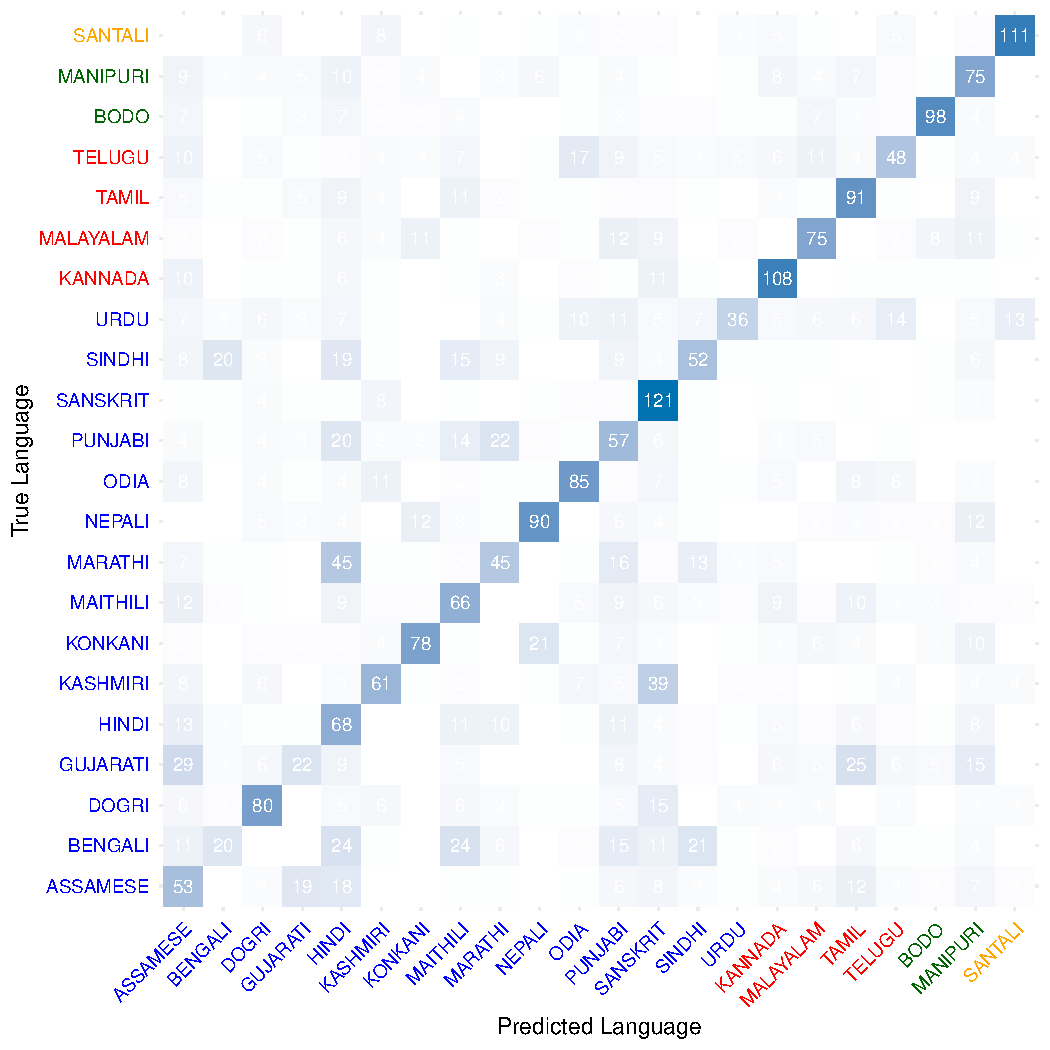
\includegraphics[width=\textwidth]{figures/confusion_matrix_raw_ordered.pdf}
         \caption{Baseline (No Correction)}
         \label{fig:conf_baseline}
     \end{subfigure}
     \hfill
     \begin{subfigure}[b]{0.48\textwidth}
         \centering
         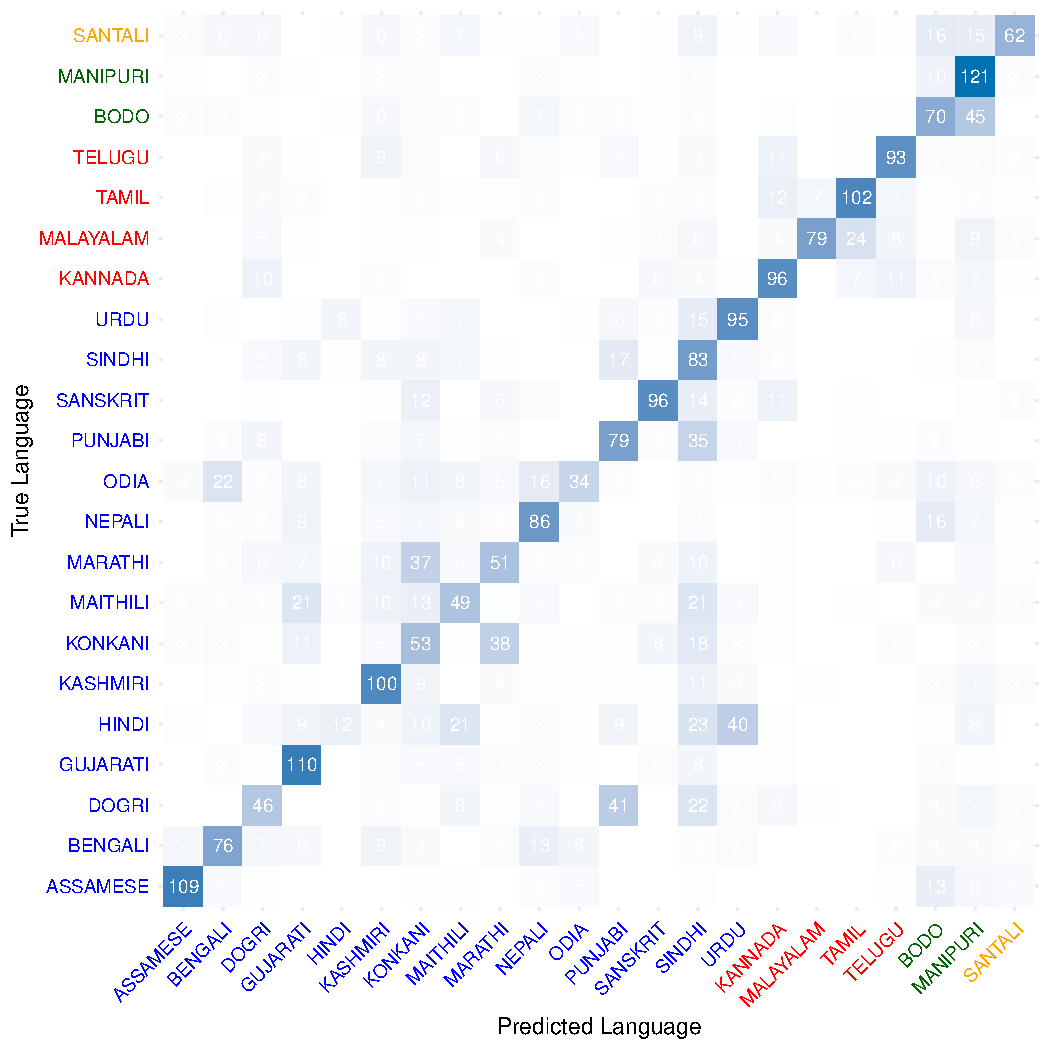
\includegraphics[width=\textwidth]{figures/confusion_matrix_knn_ordered.pdf}
         \caption{kNN-VC}
         \label{fig:conf_aug}
     \end{subfigure}

     \vspace{0.5cm}

     \begin{subfigure}[b]{0.48\textwidth}
         \centering
         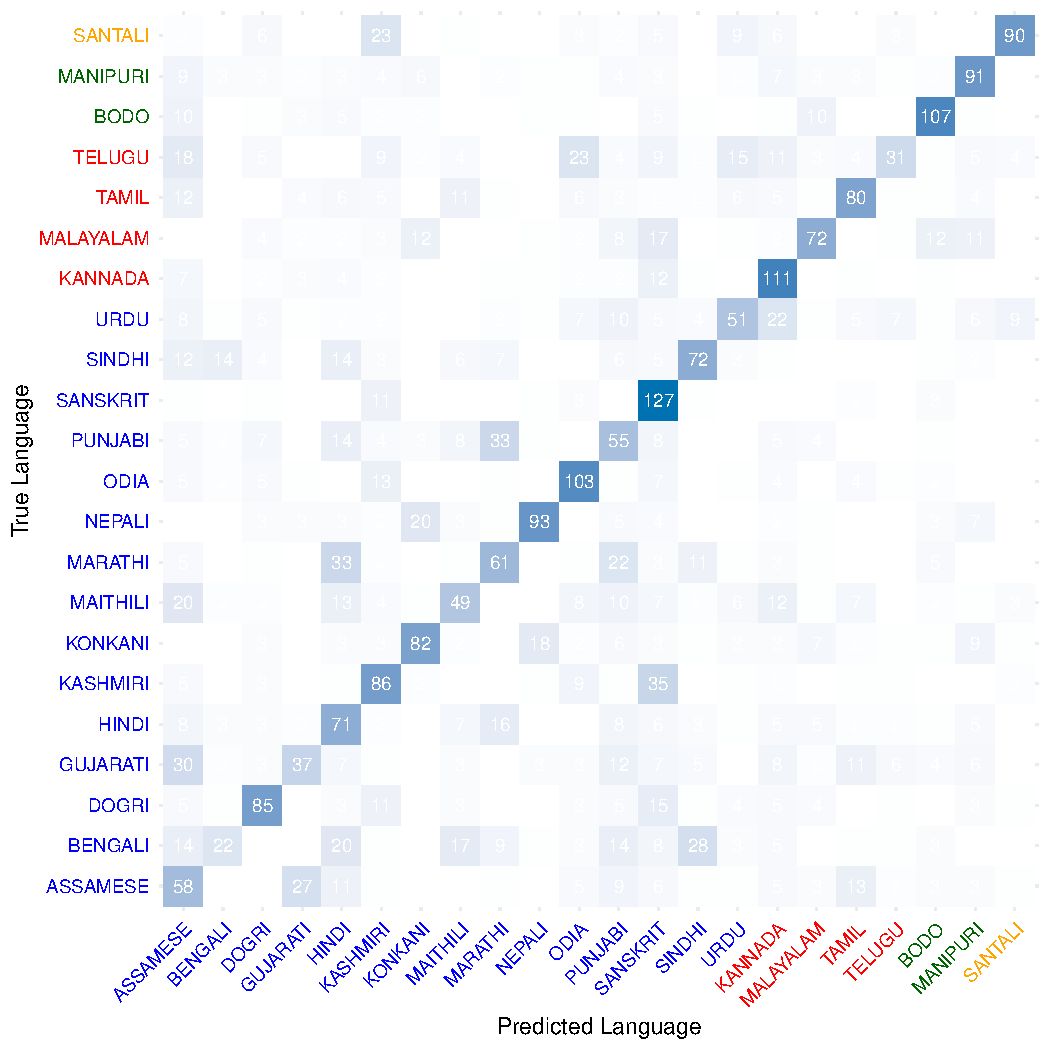
\includegraphics[width=\textwidth]{figures/confusion_matrix_DA_ordered.pdf}
         \caption{Data Augmentation}
         \label{fig:conf_knn_2} % Label geändert wegen Duplikat
     \end{subfigure}

     % \caption{\footnotesize Figure 1: Comparison of Confusion Matrices. The color-coded axes represent language families (Blue: Indo-Aryan, Red: Dravidian, Green: Tibeto-Burman, Yellow: Austroasiatic)}
     % \label{fig:comparison_plots}
\end{figure}

\clearpage

% --- Seite 2: t-SNE Plots ---
\begin{figure}[t]
     \centering
     \begin{subfigure}[b]{0.48\textwidth}
         \centering
         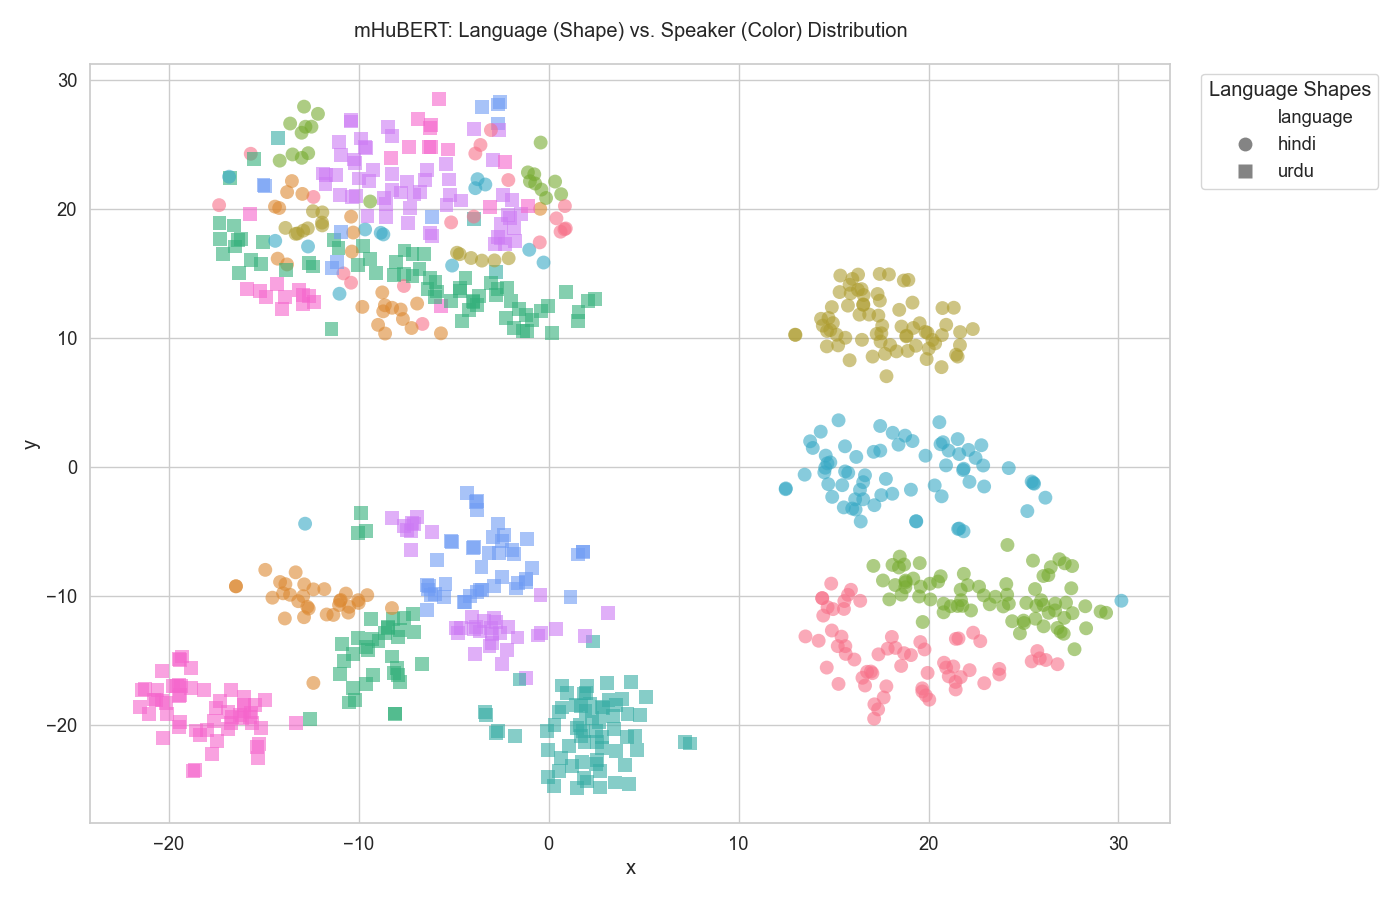
\includegraphics[width=\textwidth]{figures/HINDI-URDU_biased.png}
         \caption{biased}
         \label{fig:biased}
     \end{subfigure}
     \hfill
     \begin{subfigure}[b]{0.48\textwidth}
         \centering
         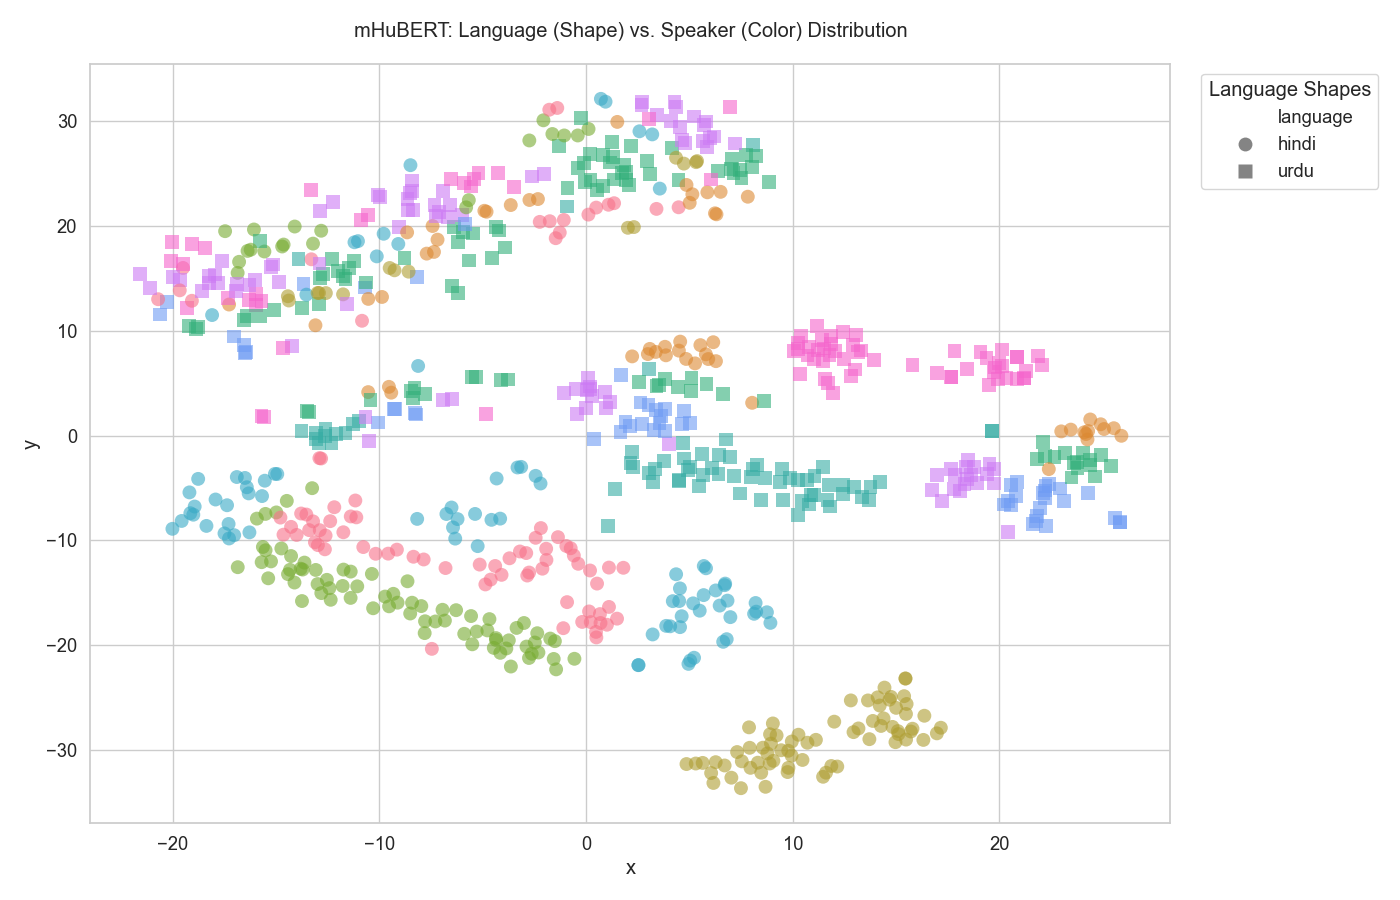
\includegraphics[width=\textwidth]{figures/HINDI-URDU_CORRECTED.png}
         \caption{biased corrected (with kNN-VC)}
         \label{fig:bias_corrected}
     \end{subfigure}
     \caption{Comparison of t-SNEs before and after bias correction with kNN-VC. Plots are colored after Speaker ID and shapes correspond to languages (Hindi = circle, Urdu = square)}
     \label{fig:tsnes}
\end{figure}
% Entries for the entire Anthology, followed by custom entries
\bibliography{custom}
\bibliographystyle{acl_natbib}

\clearpage
\appendix
\onecolumn

\renewcommand{\thefigure}{S\arabic{figure}}
\setcounter{figure}{0}

\section{Supplementary Figures}
\label{sec:appendix}
\begin{figure}[H]
    \centering
    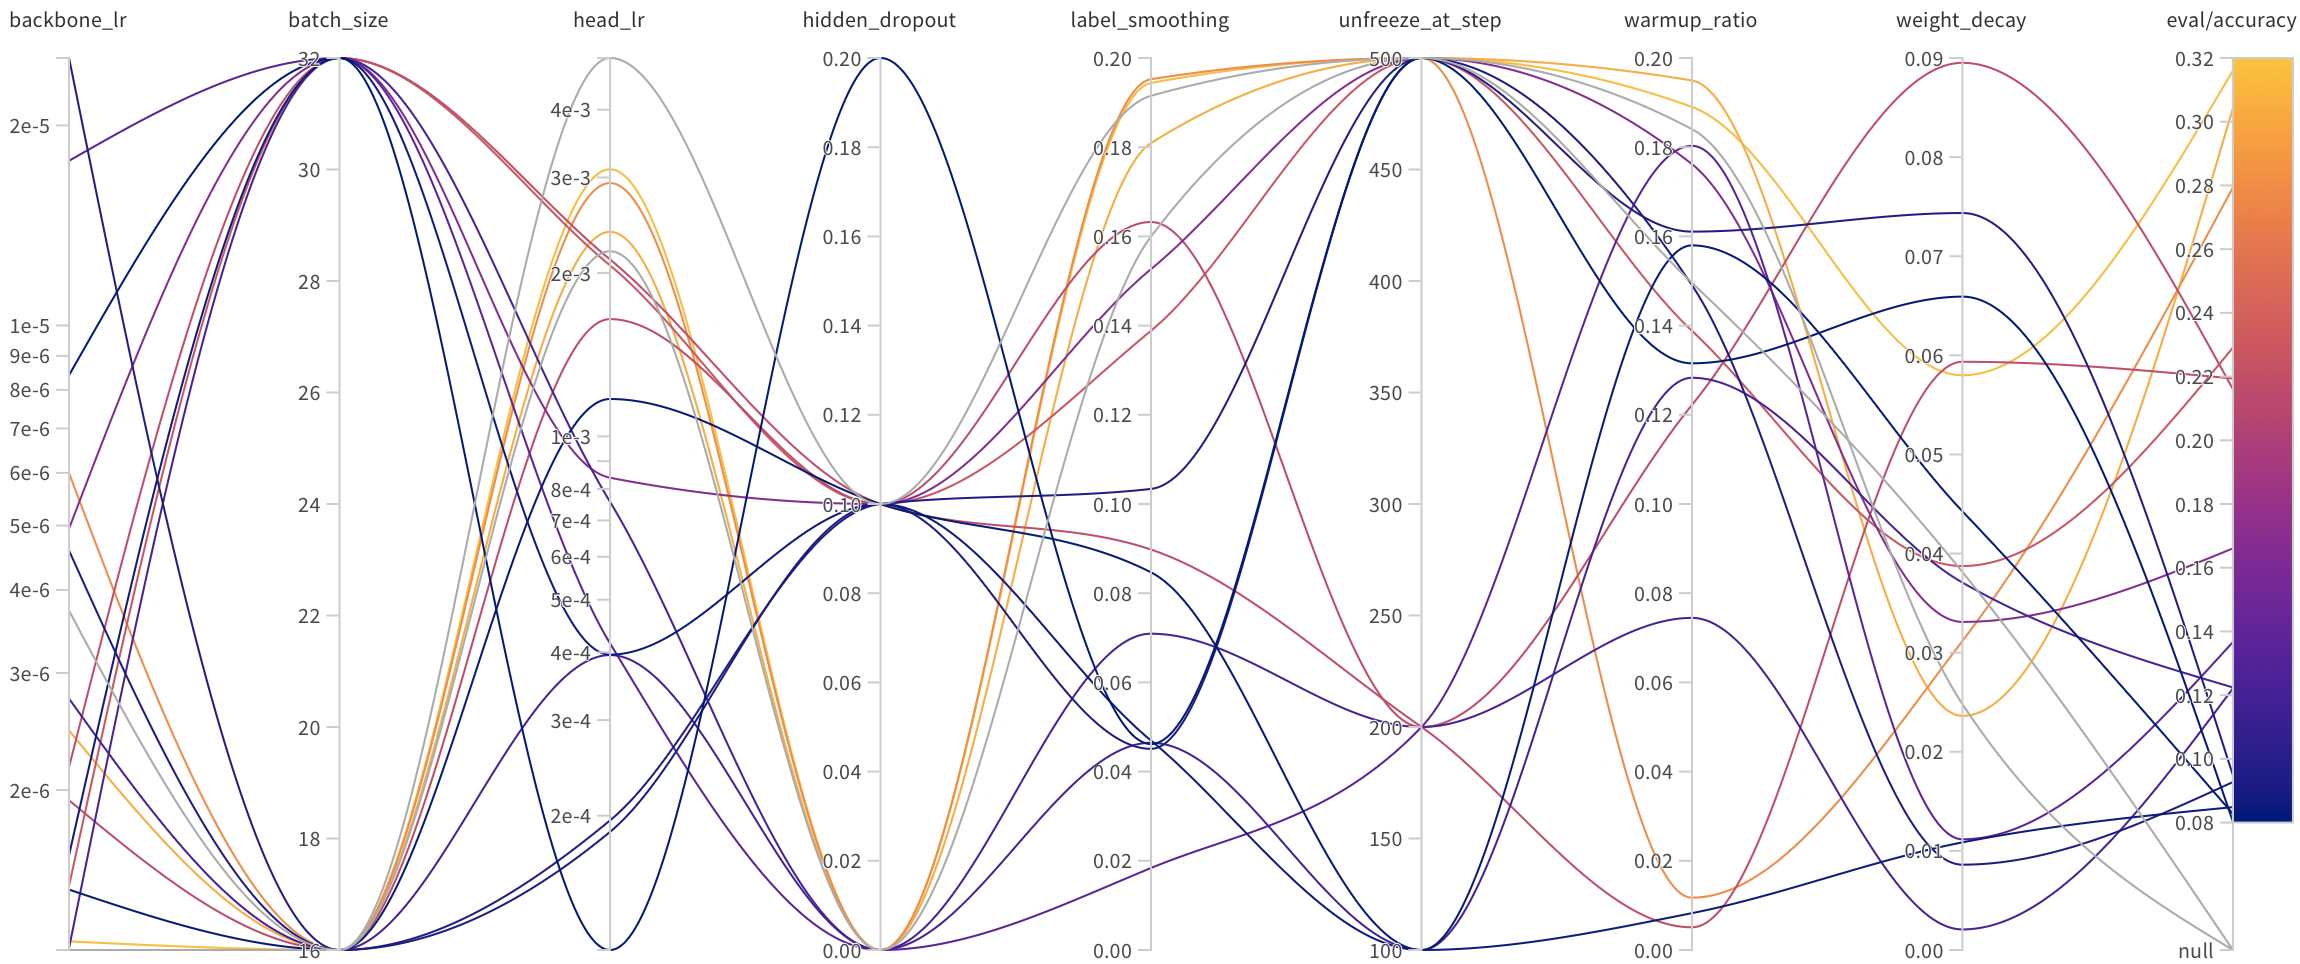
\includegraphics[width=\textwidth]{figures/WB_Sweeps.png}
    \caption{Wandb sweeps}
    \label{fig:wandb_sweeps}
\end{figure}
\begin{figure}[H]
     \centering
     % --- Linkes Bild ---
     \begin{subfigure}[b]{0.48\textwidth}
         \centering
         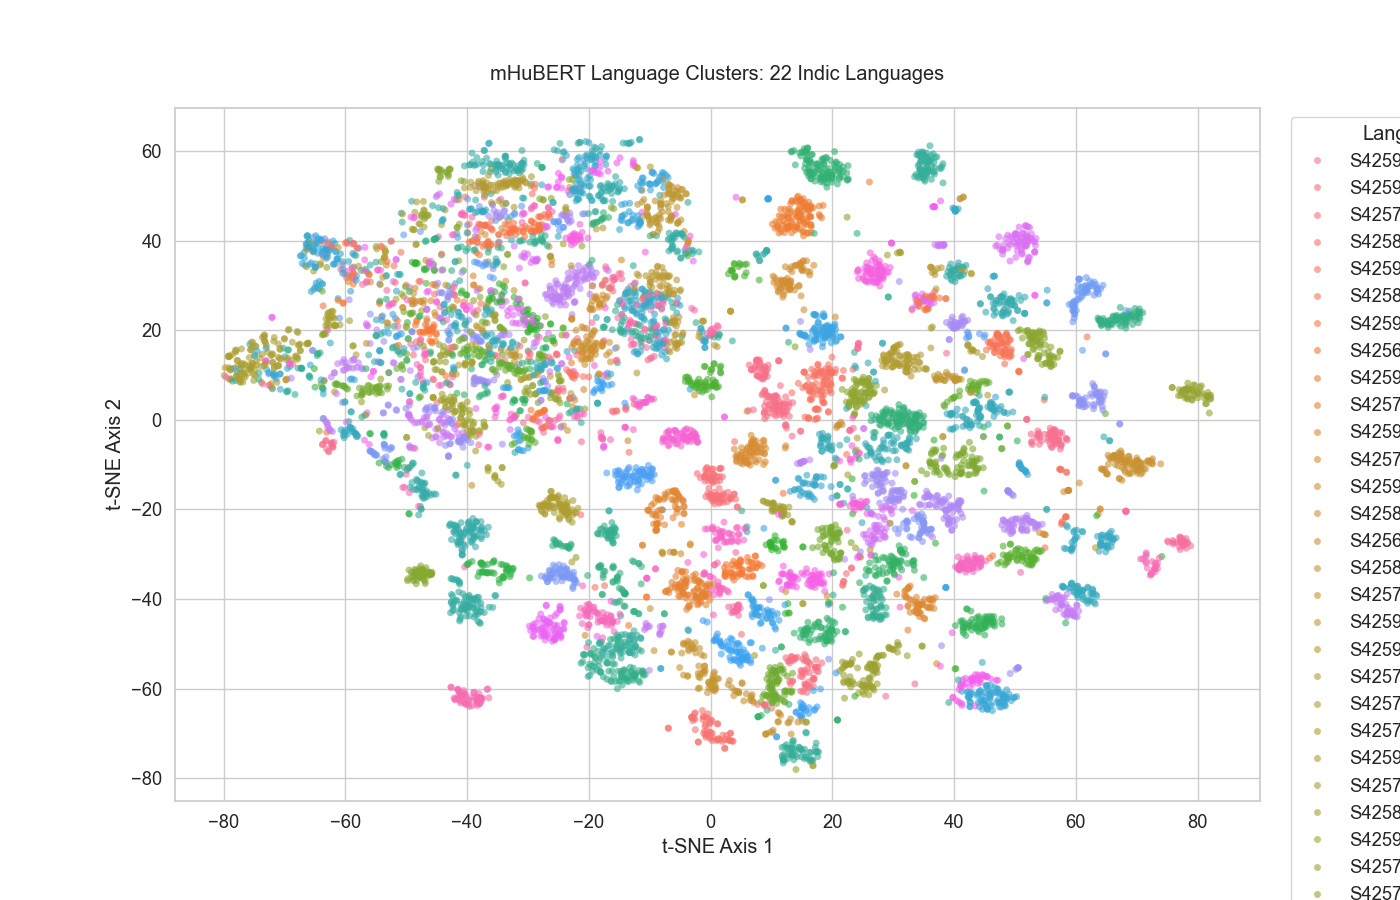
\includegraphics[width=\textwidth]{figures/bias_speakerID_tSNE.png}
         \caption{biased}
         \label{fig:S1_a}
     \end{subfigure}
     \hfill % Erzeugt den Abstand zwischen den Bildern
     % --- Rechtes Bild ---
     \begin{subfigure}[b]{0.48\textwidth}
         \centering
         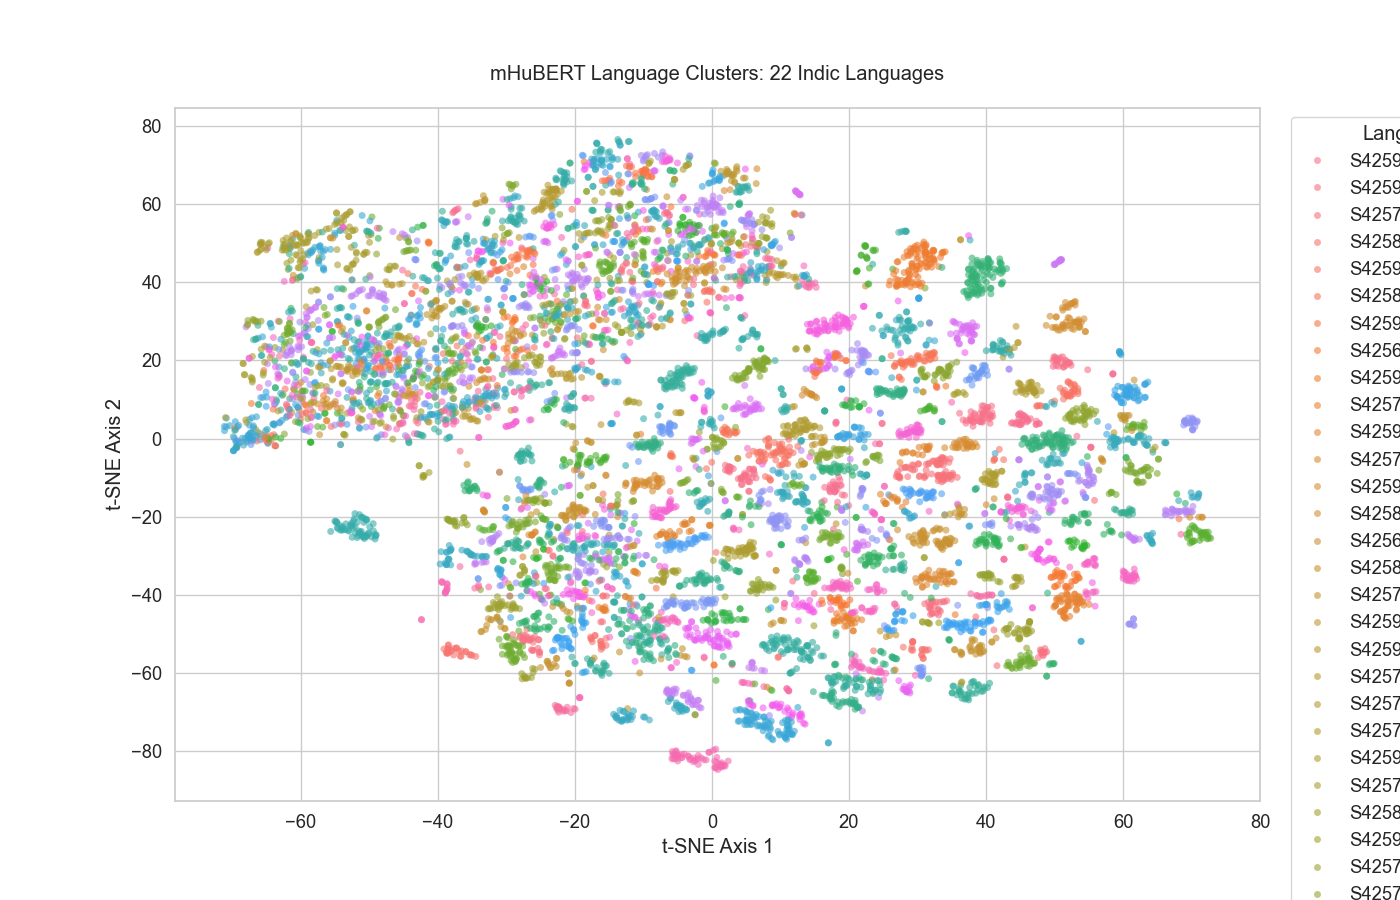
\includegraphics[width=\textwidth]{figures/corrected_speakerID_tSNE.png}
         \caption{biased corrected (with kNN-VC)}
         \label{fig:S1_b}
     \end{subfigure}
     
     \caption{t-SNE plots colored by Speaker ID)}
     \label{fig:gesamtbild}
\end{figure}
\begin{figure}[H]
     \centering
     % --- Linkes Bild ---
     \begin{subfigure}[b]{0.48\textwidth}
         \centering
         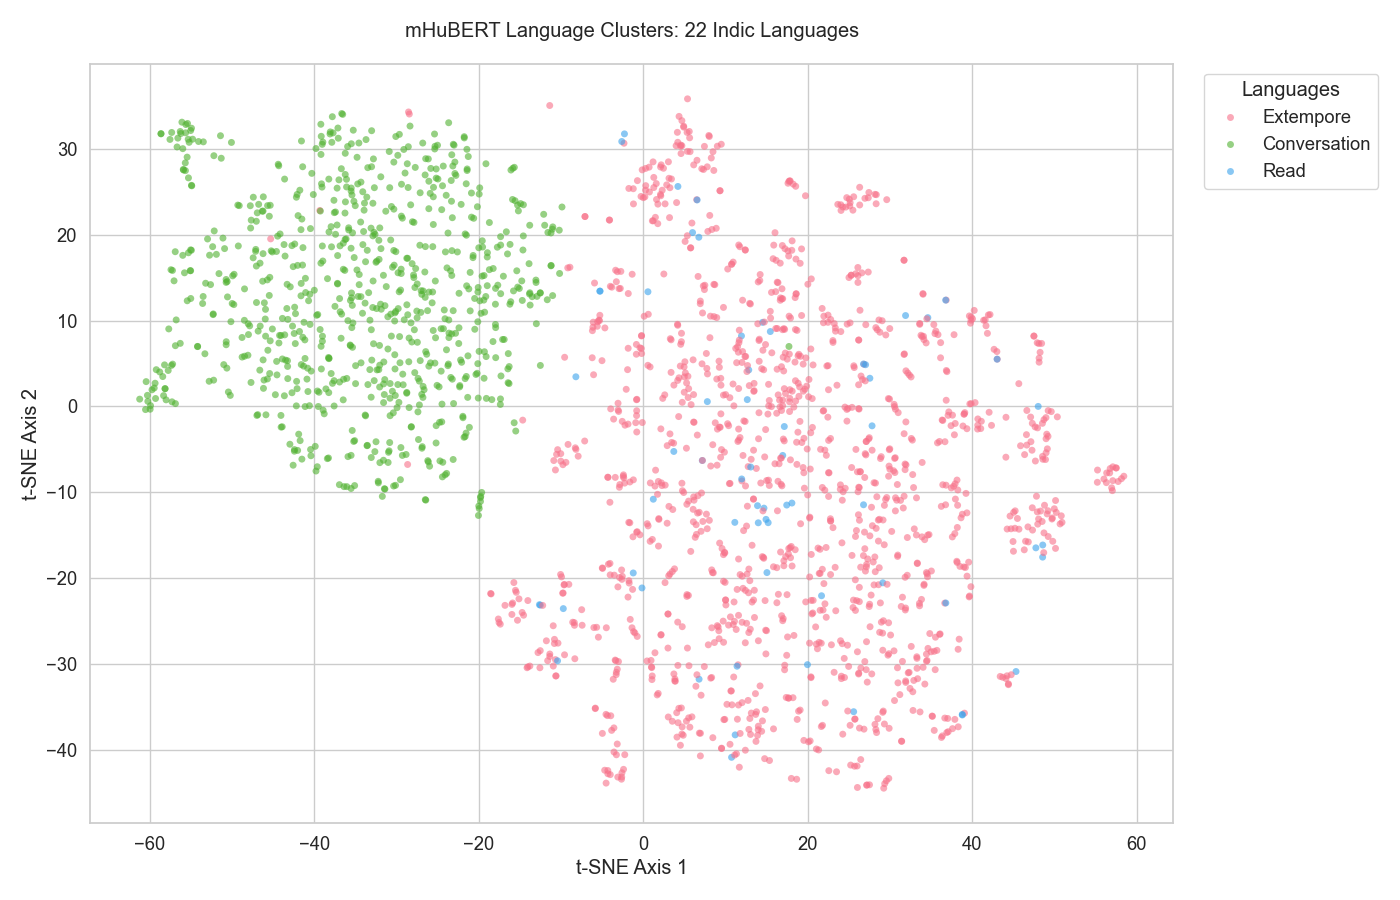
\includegraphics[width=\textwidth]{figures/Sampled_Bias_scenario_TSNE.png}
         \caption{biased}
         \label{fig:links}
     \end{subfigure}
     \hfill % Erzeugt den Abstand zwischen den Bildern
     % --- Rechtes Bild ---
     \begin{subfigure}[b]{0.48\textwidth}
         \centering
         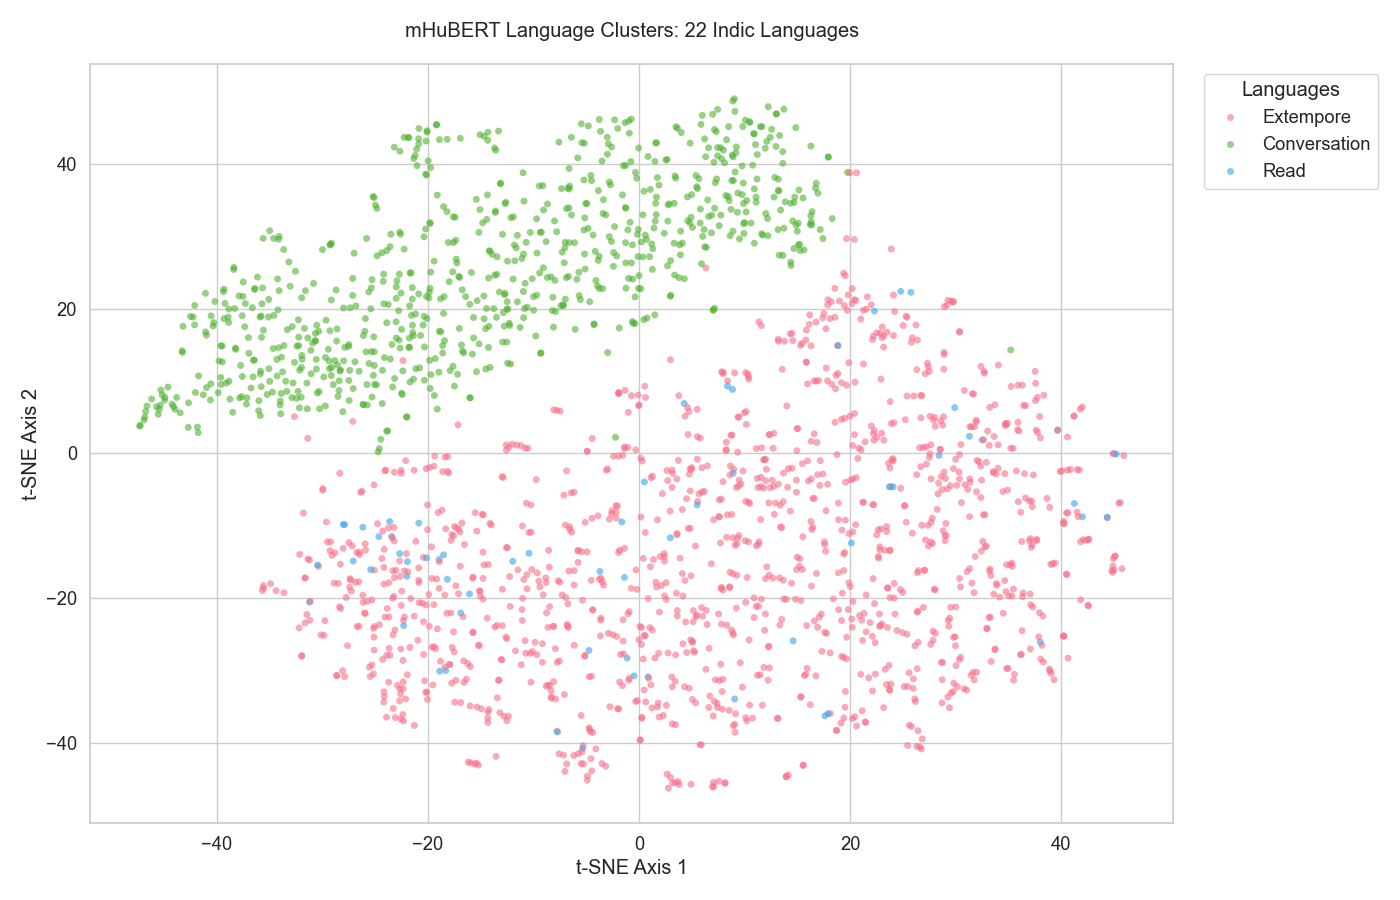
\includegraphics[width=\textwidth]{figures/Sampled_corrected_Scenario_TSNE.png}
         \caption{biased corrected (with kNN-VC)}
         \label{fig:rechts}
     \end{subfigure}
     
     \caption{t-SNE plots colored by scenario (Extempore red, Conversation green, Read blue)}
     \label{fig:gesamtbild}
\end{figure}
\begin{figure}[H]
    \begin{minipage}{0.45\textwidth} 
        \centering
        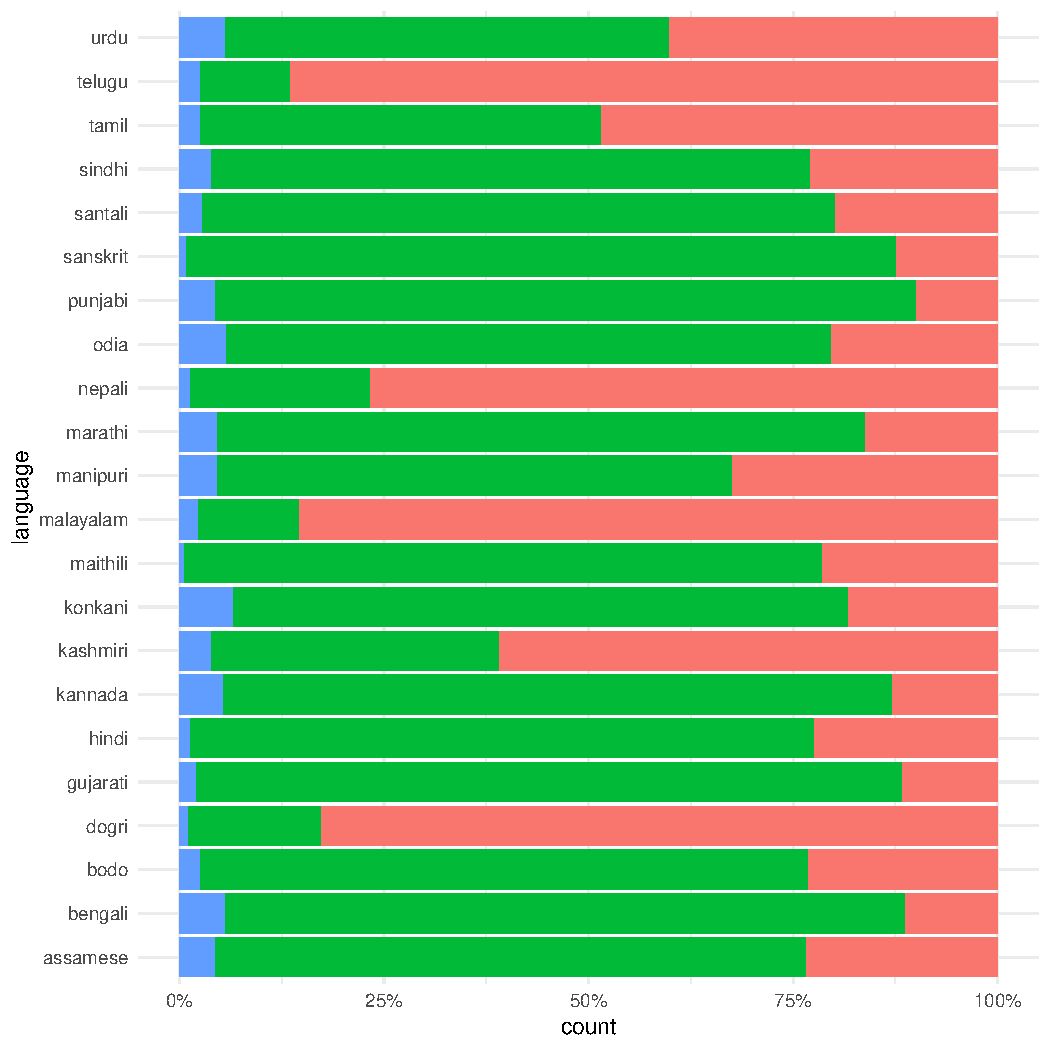
\includegraphics[width=\textwidth]{figures/scenario.pdf}
        \caption{Distribution of scenarios among all language classes (Extempore red, Conversation green, Read blue).\label{fig:scenario}}
    \end{minipage}
    \begin{minipage}{0.45\textwidth} 
        \centering
        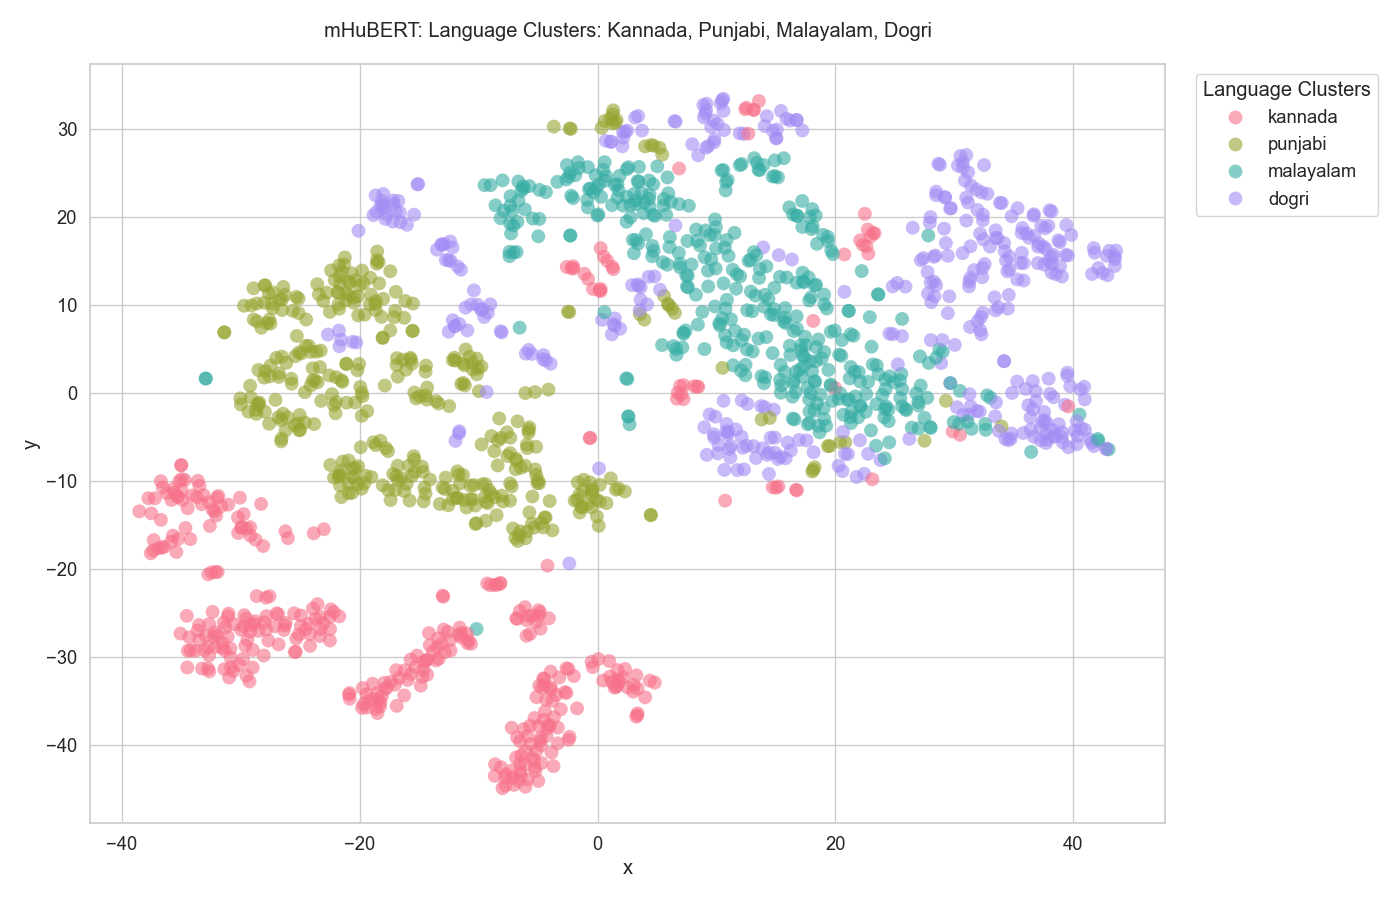
\includegraphics[width=\textwidth]{figures/bias_corrected_4lang.png}
        \caption{Clustering of languages with similar number of Conversation samples (Kannada, Punjabi) vs languages with similar number of extempore samples (Malayalam, Dogri).\label{fig:4lang}}
    \end{minipage}
\end{figure}

\begin{figure}[H]
    \centering
    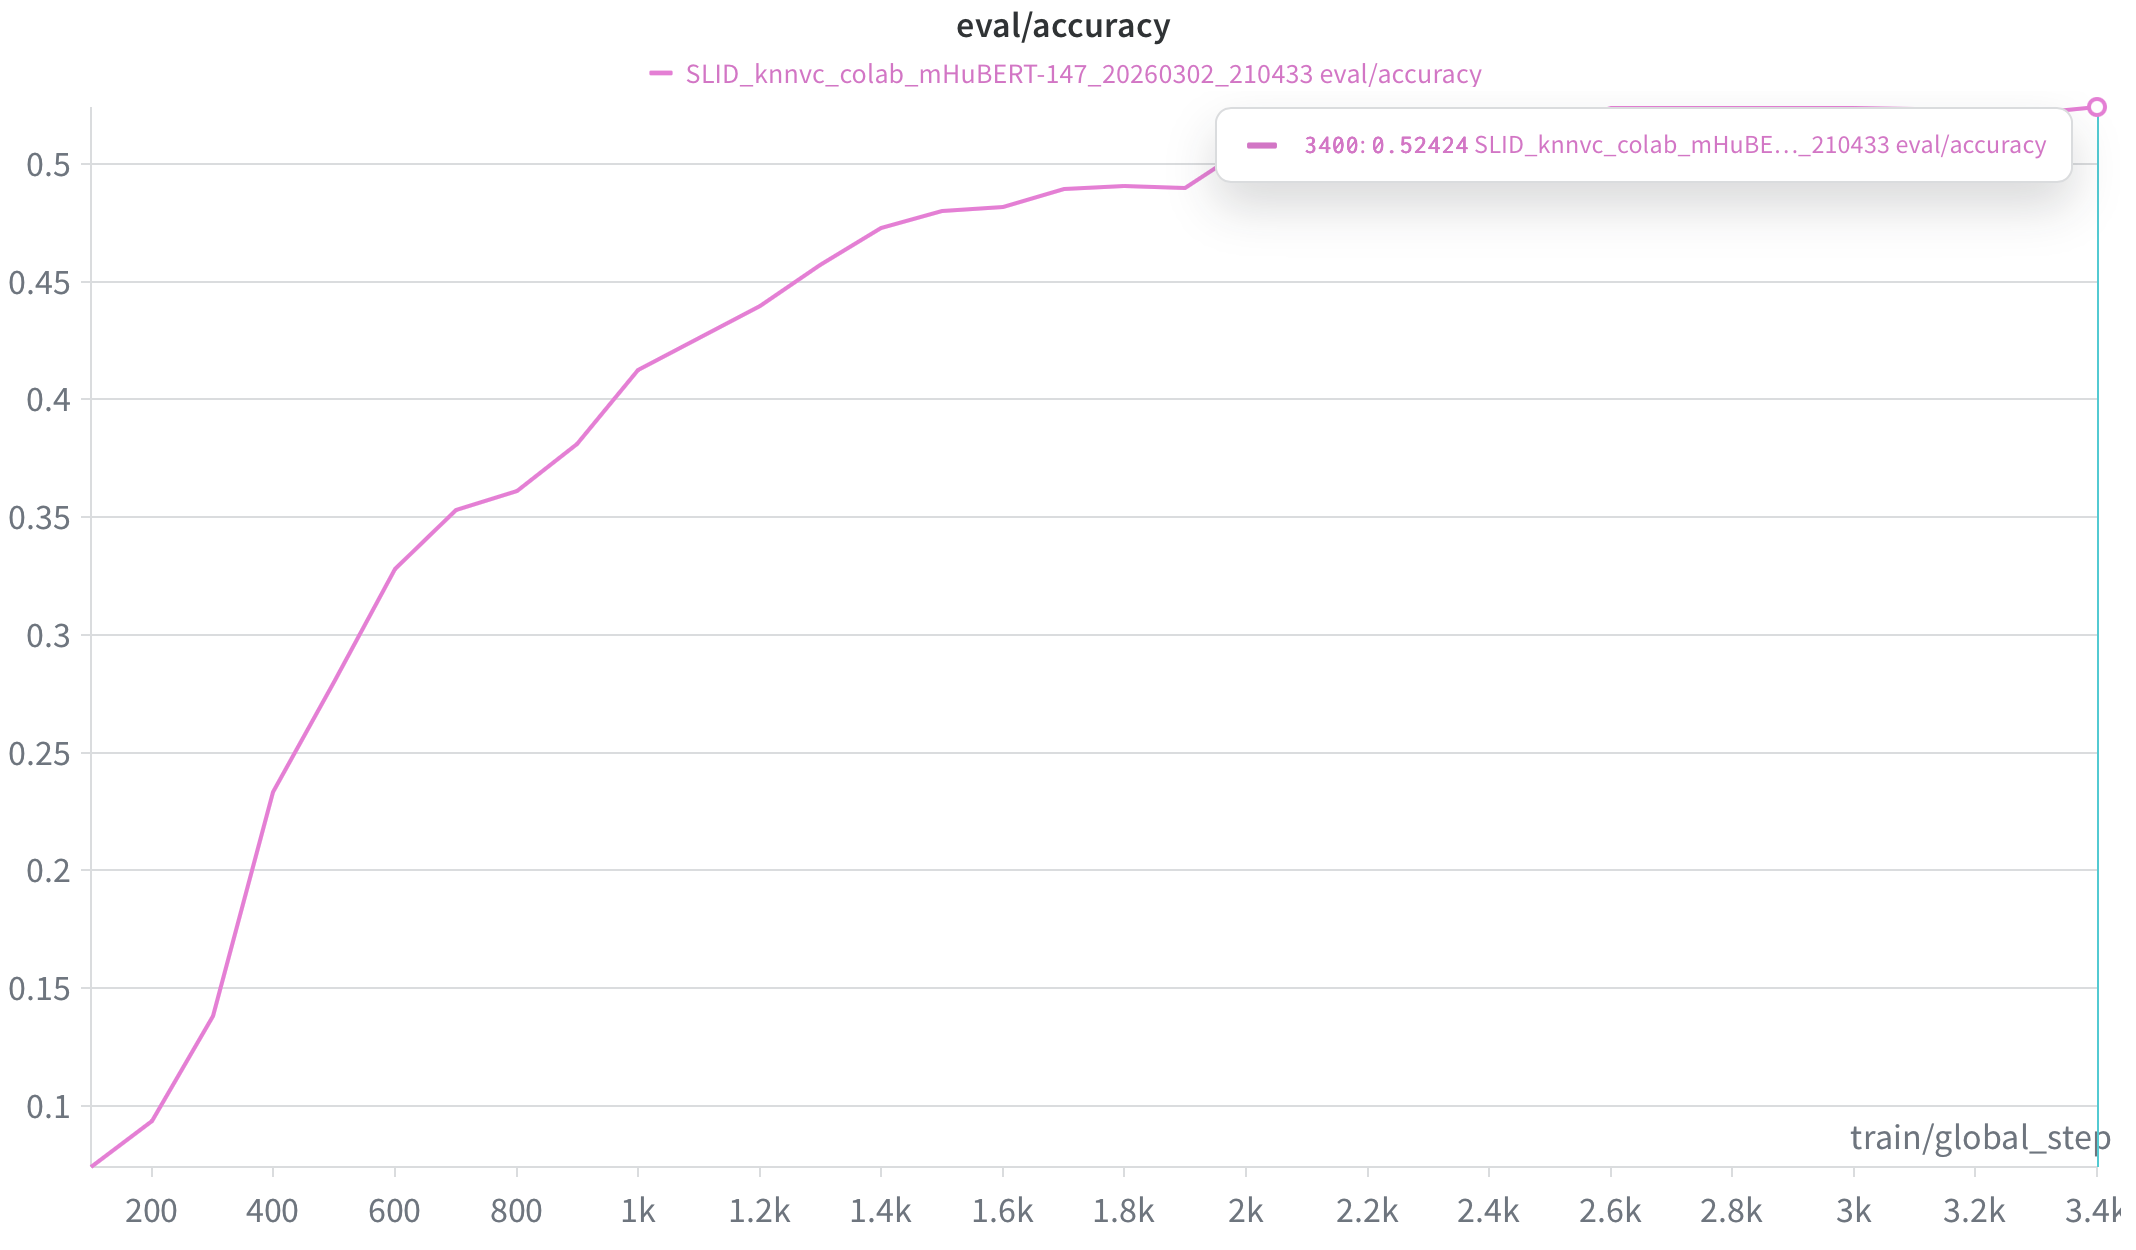
\includegraphics[width=\textwidth]{figures/WB_best_accuracy.png}
    \caption{Wandb best model accuracy}
    \label{fig:wandb_best_model_accuracy}
\end{figure}


\end{document}
